\newcommand{\defs}{../defs}
\documentclass[12pt,oneside,chapterprefix=true]{scrbook}

\usepackage[T1]{fontenc}
\usepackage[utf8x]{inputenc}
\usepackage[brazilian]{babel}
\usepackage[table]{xcolor}
\usepackage{minted}
\usepackage[a5paper,left=0.7cm,right=0.7cm,top=2cm,bottom=2.5cm,]{geometry}
\usepackage{url}
\usepackage{graphicx}
\usepackage[export]{adjustbox}
\usepackage{hyperref}
\usepackage[square]{natbib}
\usepackage[parfill]{parskip}
\usepackage{mdframed}
\usepackage{longtable}
\usepackage{soul}
\usepackage{tabularx}
\usepackage[shortlabels]{enumitem}
\usepackage{xifthen}
\usepackage{multirow}
\usepackage[portuguese, ruled, vlined, linesnumbered, algochapter]{algorithm2e}
\usepackage{amsmath}
\usepackage{amssymb}
\usepackage{amsthm}
\usepackage{tablefootnote}
\usepackage{subfigure}
\usepackage{gensymb}
\usepackage{pgfplots}
\usepackage{xpatch}
\usepackage{varwidth}
\usepackage[htt]{hyphenat}

\renewcommand{\familydefault}{\sfdefault}

\newcommand{\name}{Prof. Marcelo de Souza}
\newcommand{\email}{marcelo.desouza@udesc.br}
\newcommand{\course}{Bacharelado em Engenharia de Software}
\newcommand{\university}{Universidade do Estado de Santa Catarina}
\newcommand{\campus}{Centro de Educação Superior do Alto Vale do Itajaí}
\newcommand{\shortuniversity}{UDESC Ibirama}
\newcommand{\version}{Versão compilada em \today}
\newcommand{\exercisedescription}{Exercício}

\usepackage[automark,headsepline,footsepline]{scrlayer-scrpage}
\lehead{\content}
\lohead{\content}
\rehead{}
\rohead{}
\cehead{}
\cohead{}
\lefoot{\name}
\lofoot{\name}
\refoot{\\\thepage}
\rofoot{\\\thepage}
\cofoot{}
\cefoot{}
\setkomafont{pagehead}{\normalfont\small}
\setkomafont{pagefoot}{\normalfont}

\newpairofpagestyles{firstpage}{}

\newcommand{\makeheader}{
	\thispagestyle{firstpage}
	\vspace*{-42pt}
	\framebox[\textwidth]{
		\parbox{0.97\textwidth}{
			\begin{center}
				{\scriptsize\shortcourse\ -- \class}
				
				\vspace{10pt}
				
				\textbf{\content}
				
				\vspace{2pt}
				
				{\small\name}
				
				\vspace{10pt}
				
				{\scriptsize\shortuniversity\hfill\email}
				
				\vspace{-5pt}
				
				{\scriptsize\course\hfill\version}
				
			\end{center}
		}
	}
%	\vspace{-15pt}
%	\begin{flushright}
%		{\scriptsize\source}
%	\end{flushright}
	\smallskip
}

\renewcommand{\thesection}{\arabic{section}}

\allowdisplaybreaks

\hypersetup{
	colorlinks,
	linkcolor={blue!80!black},
	citecolor={blue!80!black},
	urlcolor={blue!80!black}
}

\definecolor{codelinecolor}{gray}{.90}
\colorlet{codeboxcolor}{blue!8}

\surroundwithmdframed{minted}

\BeforeBeginEnvironment{mdframed}{}
\AfterEndEnvironment{mdframed}{}

\mdfsetup{%
	backgroundcolor=codeboxcolor,
	linecolor=white}

\setminted{%
	mathescape,
	escapeinside=@@,
	linenos,
	breaklines,
	tabsize=3,
	fontsize=\footnotesize}

\newcommand{\code}[1]{%
	\sethlcolor{codelinecolor}
	\texttt{\hl{#1}}%
}

\newcommand{\inblock}[1]{%
	\sethlcolor{blockcolor}
	\hl{\mbox{#1}}%
}

\newcommand{\javacode}[1]{%
	\mintinline[escapeinside=~~]{java}{#1}
}

\newcommand{\javacodecolor}[1]{%
	\mintinline[escapeinside=~~,bgcolor=codeboxcolor]{java}{#1}
}

\newcounter{number}
\newenvironment{exercise}[1][]
{%
	\refstepcounter{number}%
	\noindent%
	\ifthenelse{\equal{#1}{}}%
		{\textbf{\exercisedescription~\thenumber.\\}}%
		{\textbf{\exercisedescription~\thenumber. (#1)\\}}%
	\rmfamily%
}{\medskip}%

\newcommand{\resetexercisenumbering}{
	\setcounter{number}{0}
}

\newcounter{solutionnumber}
\newenvironment{solution}[1][]
{%
	\refstepcounter{solutionnumber}%
	\noindent%
	\ifthenelse{\equal{#1}{}}%
	{\textbf{Solução -- \exercisedescription~\thesolutionnumber.\\}}%
	{\textbf{Solução -- \exercisedescription~\thesolutionnumber. (#1)\\}}%
	\rmfamily%
}{\medskip}%

\makeatletter%
\setlength{\@fptop}{5pt}

\def\arraystretch{1.5}

\newcommand{\insertspace}{\vspace{1.2em}}
\newcommand{\removespace}{\vspace{-1.2em}}

\setlength{\fboxsep}{0.8em}

\usepackage{array}
\newcolumntype{L}[1]{>{\raggedright\let\newline\\\arraybackslash\hspace{0pt}}m{#1}}
\newcolumntype{C}[1]{>{\centering\let\newline\\\arraybackslash\hspace{0pt}}m{#1}}
\newcolumntype{R}[1]{>{\raggedleft\let\newline\\\arraybackslash\hspace{0pt}}m{#1}}

\colorlet{blockcolor}{red!25}
\colorlet{redtext}{red!60!black}

\newcommand{\block}[1]{%
	\medskip
	\begin{figure}[H]
		\centering
		\begin{tikzpicture}
		\node [rectangle, align=center, fill=blockcolor, rounded corners=0.04cm, opacity = 1, text opacity = 1] {%
			#1
		};
		\end{tikzpicture}
	\end{figure}
}

\newcommand{\newtitle}[1]{%
	\begin{figure}[H]
		\begin{tikzpicture}
		\node [rectangle, fill=blue!30, rounded corners=0.04cm, opacity=1, text opacity=1, minimum width=\textwidth, text width=\linewidth-2*\pgfkeysvalueof{/pgf/inner xsep}, align=left] {%
			\textbf{#1}
		};
		\end{tikzpicture}
	\end{figure}
	\vspace{-10pt}
}

\renewcommand{\qedsymbol}{$\blacksquare$}
\xpatchcmd{\proof}{\itshape}{\normalfont\bfseries}{}{}

\newcommand{\content}{Ordenação de estruturas lineares}
\newcommand{\class}{Algoritmos e Estruturas de Dados}
\newcommand{\shortcourse}{45EST}

\begin{document}

\makeheader

{
Leitura obrigatória:
\begin{itemize}
	\item Capítulo 4 de~\cite{Ziviani2010} -- Ordenação.
\end{itemize}

Leitura complementar:
\begin{itemize}
	\item Capítulo 13 de~\cite{Pereira2008} -- Ordenação e busca.
	\item Capítulo 15 de~\cite{Preiss2001} -- Algoritmos de ordenação e ordenadores.
\end{itemize}
}

\medskip

\newtitle{Algoritmos de ordenação}

\begin{itemize}
	\item Dada uma coleção de elementos, devolve a coleção ordenada.
	
	{\color{redtext}
	\item Existem diversos algoritmos diferentes para ordenação.
	\item Veja demonstrações dos algoritmos em:
	{\fontsize{9pt}{4pt}
	\begin{itemize}
		\item \url{https://www.cs.usfca.edu/~galles/visualization/ComparisonSort.html}.
		\item \url{https://visualgo.net/en/sorting}.
	\end{itemize}
	}}
\end{itemize}

\medskip

\newtitle{Algoritmo \textit{BubbleSort}}

\begin{itemize}
	\item Algoritmo baseado em trocas.
	\item Funcionamento:
	\begin{itemize}
		\item Percorre elementos vizinhos e os inverte (\textit{swap}) quando estão fora de ordem.
		\item Na primeira passagem, maior elemento vai para última posição.
		\item Na segunda passagem, segundo maior elemento vai para penúltima posição.
		\item Etc.
	\end{itemize}
	\item Complexidade $O(n^2)$.
	\item Veja o funcionamento do algoritmo em \url{https://bit.ly/1wFxLr0}.
\end{itemize}

\medskip

Algoritmo BubbleSort:
\begin{minted}{java}
public class BubbleSort {
	public void sort(int[] array) {
		for(int i = 0; i < array.length; i++)
			for(int j = 0; j < array.length - (i + 1); j++)
				if(array[j] > array[j + 1])
					swap(j, j + 1, array);
	}
	
	private void swap(int i, int j, int[] array) {
		int temp = array[i];
		array[i] = array[j];
		array[j] = temp;
	}
}
\end{minted}

\medskip

{\color{redtext}
Comentários:
\begin{itemize}
	\item Cada vez que percorre o vetor vai até a última posição não-ordenada.
	\item Método \texttt{swap} troca elementos de posição.
\end{itemize}
}

\clearpage

\newtitle{Algoritmo \textit{SelectionSort}}

\begin{itemize}
	\item Algoritmo baseado em seleção.
	\item Funcionamento:
	\begin{itemize}
		\item Percorre a lista para encontrar o menor valor.
		\item Troca o menor valor com o primeiro elemento.
		\item Repete o processo para a sub-lista ainda não ordenada.
	\end{itemize}
	\item Complexidade $O(n^2)$.
	\item Veja o funcionamento do algoritmo em \url{https://bit.ly/1wFxLr0}.
\end{itemize}

\medskip

Algoritmo SelectionSort:
\begin{minted}{java}
public class SelectionSort {	
	public void sort(int[] array) {
		for(int i = 0; i < array.length - 1; i++) {
			int min = i;
			for(int j = i + 1; j < array.length; j++)
				if(array[j] < array[min])
					min = j;
			swap(min, i, array);
		}
	}
	
	private void swap(int i, int j, int[] array) {
		int temp = array[i];
		array[i] = array[j];
		array[j] = temp;
	}
}
\end{minted}

\medskip

{\color{redtext}
	Comentários:
	\begin{itemize}
		\item A cada iteração o menor elemento é levado para a frente.
	\end{itemize}
}

\clearpage

\newtitle{Algoritmo \textit{InsertionSort}}

\begin{itemize}
	\item Algoritmo baseado em inserção.
	\item Funcionamento:
	\begin{itemize}
		\item Em uma lista de $0$ até $n - 1$, inicializa $i = 1$.
		\item Percorre a lista de $i$ até $0$ e posiciona o elemento $i$.
		\item Incrementa $i$ e volta ao passo anterior.
	\end{itemize}
	\item Complexidade $O(n^2)$.
	\item Veja o funcionamento do algoritmo em \url{https://bit.ly/1wFxLr0}.
\end{itemize}

\medskip

\begin{figure}[H]
	\centering
	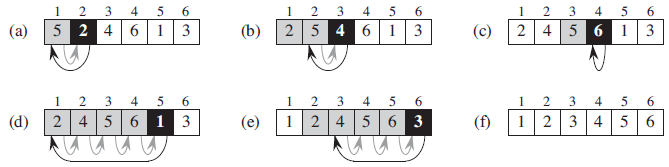
\includegraphics[width=0.85\linewidth]{img/insertion-sort}
\end{figure}

\medskip

Algoritmo InsertionSort:
\begin{minted}{java}
public class InsertionSort {
	public void sort(int[] array) {
		int temp;
		for(int i = 1; i < array.length; i++) {
			for(int j = i ; j > 0 ; j--)
				if(array[j] < array[j - 1])
					swap(j, j - 1, array);
	}
	
	private void swap(int i, int j, int[] array) {
		int temp = array[i];
		array[i] = array[j];
		array[j] = temp;
	}
}
\end{minted}

\medskip

{\color{redtext}
	Comentários:
	\begin{itemize}
		\item A cada iteração, temos a lista de $0$ até $i$ ordenada.
	\end{itemize}
}

\medskip

\newtitle{Algoritmo \textit{MergeSort}}

\begin{itemize}
	\item Algoritmo baseado no conceito de \textit{divisão e conquista}.
	\item Funcionamento:
	\begin{itemize}
		\item Iterativamente divide o vetor pela metade, até que cada parte contenha um elemento.
		\item Iterativamente junta as partes (\textit{merge}), ordenando os elementos.
	\end{itemize}
	\item Complexidade $O(n \log n)$.
	\item Veja o funcionamento do algoritmo em \url{https://bit.ly/1wFxLr0}.
\end{itemize}

\medskip

\begin{figure}[H]
	\centering
	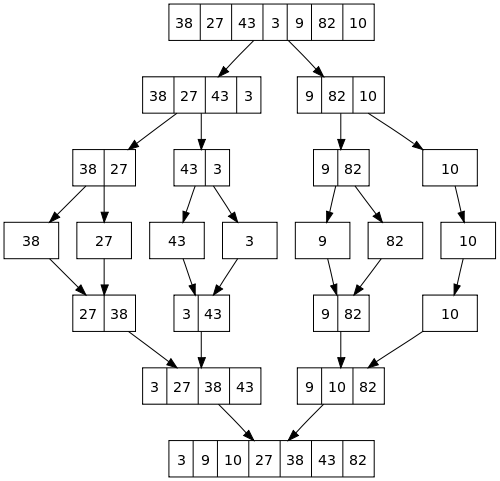
\includegraphics[width=0.47\linewidth]{img/merge-sort}
\end{figure}

\medskip

Algoritmo MergeSort:
\begin{minted}{java}
public class MergeSort {
	
	int[] tempMergArr;
	
	public void sort(int array[]) {
		tempMergArr = new int[array.length];
		mergeSort(array, 0, array.length - 1);
	}
	
	private void mergeSort(int[] array, int start, int end) {
		if (start < end) {
			int middle = start + ((end - start) / 2);
			mergeSort(array, start, middle);
			mergeSort(array, middle + 1, end);
			merge(array, start, middle, end);
		}
	}
	
	private void merge(int[] array, int start, int middle, int end) {		
		for (int i = start; i <= end; i++) {
			tempMergArr[i] = array[i];
		}
		
		int i = start;
		int j = middle + 1;
		int k = start;
		while (i <= middle && j <= end) {
			if (tempMergArr[i] <= tempMergArr[j]) {
				array[k] = tempMergArr[i];
				i++;
			} else {
				array[k] = tempMergArr[j];
				j++;
			}
			k++;
		}

		while (i <= middle) {
			array[k] = tempMergArr[i];
			k++;
			i++;
		}
		while (j <= end) {
			array[k] = tempMergArr[j];
			k++;
			j++;
		}		
	}
}
\end{minted}
	
\medskip

{\color{redtext}
	Comentários:
	\begin{itemize}
		\item O método \texttt{mergeSort} é chamado recursivamente com as duas metades, até ser chamado com um único elemento (divisão).
		\item Após isso, cada parte é jutada pelo método \texttt{merge}.
		\item Na junção, o algoritmo insere no vetor os elementos ordenados das duas metades.
		\item Faça um teste de mesa para verificar o funcionamento do \textit{merge sort}.
	\end{itemize}
}

\medskip

\newtitle{Atividades}

\begin{enumerate}
	\item Pesquise a respeito de outros algoritmos de ordenação:
	\begin{enumerate}[a.]
		\item Quick sort
		\item Shell sort
		\item Radix sort
		\item Bucket sort
	\end{enumerate}
	
	\item No algoritmo \textit{bubble sort}, se em uma iteração intermediária o vetor for percorrido sem nenhuma troca, significa que os elementos já estão ordenados. Neste caso, não é necessário seguir as próximas etapas do algoritmo. Faça as modificações necessárias para implementar esta estratégia.
	
	\item Modifique o algoritmo \texttt{InsertionSort} para que ele execute uma busca binária para encontrar a posição de inserção do elemento. Qual a nova complexidade do algoritmo?
	
	\item Considere uma matriz retangular. Ordene os elementos de cada linha. Após isso, ordene os elementos de cada coluna. A primeira ordenação foi perdida? Por que?
	
	\item Cada redação do Enem é corrigida por três professores diferentes. A nota final consiste na média aritmética das três notas. Crie um programa para ler as notas de todas as redações e armazenar as médias em um vetor. Ao final, aplique um algoritmo de ordenação nesta estrutura e apresente as dez maiores notas.
	
	\item Modifique o exercício anterior, de modo que sejam armazenadas mais informações de cada redação: nome do aluno, RG do aluno, notas dos professores e média final.
\end{enumerate}

\medskip

\newtitle{Referências}
\begingroup
	\footnotesize
	\renewcommand{\chapter}[2]{}%
	\bibliographystyle{apalike}
	\bibliography{../referencias}
\endgroup

\end{document}